\documentclass[pdf, unicode, 9pt, notheorems, handout]{beamer}

%\mode<handout> {
%    \usepackage{pgfpages}
%    \setbeameroption{show notes}
%    \pgfpagesuselayout{2 on 1}[a4paper, border shrink=5mm]
%    \setbeamercolor{note page}{bg=white}
%    \setbeamercolor{note title}{bg=gray!10}
%    \setbeamercolor{note date}{fg=gray!10}
%}

\usepackage[utf8]{inputenc}
\usepackage[T2A]{fontenc}
\usepackage[russian, english]{babel}
\usepackage{ragged2e}
%\usepackage{t-angles}
%\usepackage{slashbox}
\usepackage{hhline}
\usepackage{slashbox}
\usepackage{tikz}
\usetikzlibrary{tikzmark, calc, fit}
\usepackage{beamerthemesplit}

%new calligraphic font for subspaces 
\usepackage{euscript}
\newcommand{\cA}{\EuScript{A}}
\newcommand{\cB}{\EuScript{B}}
\newcommand{\cC}{\EuScript{C}}
\newcommand{\cD}{\EuScript{D}}
\newcommand{\cE}{\EuScript{E}}
\newcommand{\cF}{\EuScript{F}}
\newcommand{\cG}{\EuScript{G}}
\newcommand{\cH}{\EuScript{H}}
\newcommand{\cI}{\EuScript{I}}
\newcommand{\cJ}{\EuScript{J}}
\newcommand{\cK}{\EuScript{K}}
\newcommand{\cL}{\EuScript{L}}
\newcommand{\cM}{\EuScript{M}}
\newcommand{\cN}{\EuScript{N}}
\newcommand{\cO}{\EuScript{O}}
\newcommand{\cP}{\EuScript{P}}
\newcommand{\cQ}{\EuScript{Q}}
\newcommand{\cR}{\EuScript{R}}
\newcommand{\cS}{\EuScript{S}}
\newcommand{\cT}{\EuScript{T}}
\newcommand{\cU}{\EuScript{U}}
\newcommand{\cV}{\EuScript{V}}
\newcommand{\cW}{\EuScript{W}}
\newcommand{\cX}{\EuScript{X}}
\newcommand{\cY}{\EuScript{Y}}
\newcommand{\cZ}{\EuScript{Z}}

%font for text indices like transposition X^\mathrm{T}
\newcommand{\rmA}{\mathrm{A}}
\newcommand{\rmB}{\mathrm{B}}
\newcommand{\rmC}{\mathrm{C}}
\newcommand{\rmD}{\mathrm{D}}
\newcommand{\rmE}{\mathrm{E}}
\newcommand{\rmF}{\mathrm{F}}
\newcommand{\rmG}{\mathrm{G}}
\newcommand{\rmH}{\mathrm{H}}
\newcommand{\rmI}{\mathrm{I}}
\newcommand{\rmJ}{\mathrm{J}}
\newcommand{\rmK}{\mathrm{K}}
\newcommand{\rmL}{\mathrm{L}}
\newcommand{\rmM}{\mathrm{M}}
\newcommand{\rmN}{\mathrm{N}}
\newcommand{\rmO}{\mathrm{O}}
\newcommand{\rmP}{\mathrm{P}}
\newcommand{\rmQ}{\mathrm{Q}}
\newcommand{\rmR}{\mathrm{R}}
\newcommand{\rmS}{\mathrm{S}}
\newcommand{\rmT}{\mathrm{T}}
\newcommand{\rmU}{\mathrm{U}}
\newcommand{\rmV}{\mathrm{V}}
\newcommand{\rmW}{\mathrm{W}}
\newcommand{\rmX}{\mathrm{X}}
\newcommand{\rmY}{\mathrm{Y}}
\newcommand{\rmZ}{\mathrm{Z}}

%tt font for time series
\newcommand{\tA}{\mathsf{A}}
\newcommand{\tB}{\mathsf{B}}
\newcommand{\tC}{\mathsf{C}}
\newcommand{\tD}{\mathsf{D}}
\newcommand{\tE}{\mathsf{E}}
\newcommand{\tF}{\mathsf{F}}
\newcommand{\tG}{\mathsf{G}}
\newcommand{\tH}{\mathsf{H}}
\newcommand{\tI}{\mathsf{I}}
\newcommand{\tJ}{\mathsf{J}}
\newcommand{\tK}{\mathsf{K}}
\newcommand{\tL}{\mathsf{L}}
\newcommand{\tM}{\mathsf{M}}
\newcommand{\tN}{\mathsf{N}}
\newcommand{\tO}{\mathsf{O}}
\newcommand{\tP}{\mathsf{P}}
\newcommand{\tQ}{\mathsf{Q}}
\newcommand{\tR}{\mathsf{R}}
\newcommand{\tS}{\mathsf{S}}
\newcommand{\tT}{\mathsf{T}}
\newcommand{\tU}{\mathsf{U}}
\newcommand{\tV}{\mathsf{V}}
\newcommand{\tW}{\mathsf{W}}
\newcommand{\tX}{\mathsf{X}}
\newcommand{\tY}{\mathsf{Y}}
\newcommand{\tZ}{\mathsf{Z}}

%bf font for matrices
\newcommand{\bfA}{\mathbf{A}}
\newcommand{\bfB}{\mathbf{B}}
\newcommand{\bfC}{\mathbf{C}}
\newcommand{\bfD}{\mathbf{D}}
\newcommand{\bfE}{\mathbf{E}}
\newcommand{\bfF}{\mathbf{F}}
\newcommand{\bfG}{\mathbf{G}}
\newcommand{\bfH}{\mathbf{H}}
\newcommand{\bfI}{\mathbf{I}}
\newcommand{\bfJ}{\mathbf{J}}
\newcommand{\bfK}{\mathbf{K}}
\newcommand{\bfL}{\mathbf{L}}
\newcommand{\bfM}{\mathbf{M}}
\newcommand{\bfN}{\mathbf{N}}
\newcommand{\bfO}{\mathbf{O}}
\newcommand{\bfP}{\mathbf{P}}
\newcommand{\bfQ}{\mathbf{Q}}
\newcommand{\bfR}{\mathbf{R}}
\newcommand{\bfS}{\mathbf{S}}
\newcommand{\bfT}{\mathbf{T}}
\newcommand{\bfU}{\mathbf{U}}
\newcommand{\bfV}{\mathbf{V}}
\newcommand{\bfW}{\mathbf{W}}
\newcommand{\bfX}{\mathbf{X}}
\newcommand{\bfY}{\mathbf{Y}}
\newcommand{\bfZ}{\mathbf{Z}}

%bb font for standard spaces and expectation
\newcommand{\bbA}{\mathbb{A}}
\newcommand{\bbB}{\mathbb{B}}
\newcommand{\bbC}{\mathbb{C}}
\newcommand{\bbD}{\mathbb{D}}
\newcommand{\bbE}{\mathbb{E}}
\newcommand{\bbF}{\mathbb{F}}
\newcommand{\bbG}{\mathbb{G}}
\newcommand{\bbH}{\mathbb{H}}
\newcommand{\bbI}{\mathbb{I}}
\newcommand{\bbJ}{\mathbb{J}}
\newcommand{\bbK}{\mathbb{K}}
\newcommand{\bbL}{\mathbb{L}}
\newcommand{\bbM}{\mathbb{M}}
\newcommand{\bbN}{\mathbb{N}}
\newcommand{\bbO}{\mathbb{O}}
\newcommand{\bbP}{\mathbb{P}}
\newcommand{\bbQ}{\mathbb{Q}}
\newcommand{\bbR}{\mathbb{R}}
\newcommand{\bbS}{\mathbb{S}}
\newcommand{\bbT}{\mathbb{T}}
\newcommand{\bbU}{\mathbb{U}}
\newcommand{\bbV}{\mathbb{V}}
\newcommand{\bbW}{\mathbb{W}}
\newcommand{\bbX}{\mathbb{X}}
\newcommand{\bbY}{\mathbb{Y}}
\newcommand{\bbZ}{\mathbb{Z}}

%got font for any case
\newcommand{\gA}{\mathfrak{A}}
\newcommand{\gB}{\mathfrak{B}}
\newcommand{\gC}{\mathfrak{C}}
\newcommand{\gD}{\mathfrak{D}}
\newcommand{\gE}{\mathfrak{E}}
\newcommand{\gF}{\mathfrak{F}}
\newcommand{\gG}{\mathfrak{G}}
\newcommand{\gH}{\mathfrak{H}}
\newcommand{\gI}{\mathfrak{I}}
\newcommand{\gJ}{\mathfrak{J}}
\newcommand{\gK}{\mathfrak{K}}
\newcommand{\gL}{\mathfrak{L}}
\newcommand{\gM}{\mathfrak{M}}
\newcommand{\gN}{\mathfrak{N}}
\newcommand{\gO}{\mathfrak{O}}
\newcommand{\gP}{\mathfrak{P}}
\newcommand{\gQ}{\mathfrak{Q}}
\newcommand{\gR}{\mathfrak{R}}
\newcommand{\gS}{\mathfrak{S}}
\newcommand{\gT}{\mathfrak{T}}
\newcommand{\gU}{\mathfrak{U}}
\newcommand{\gV}{\mathfrak{V}}
\newcommand{\gW}{\mathfrak{W}}
\newcommand{\gX}{\mathfrak{X}}
\newcommand{\gY}{\mathfrak{Y}}
\newcommand{\gZ}{\mathfrak{Z}}

%old calligraphic font
\newcommand{\calA}{\mathcal{A}}
\newcommand{\calB}{\mathcal{B}}
\newcommand{\calC}{\mathcal{C}}
\newcommand{\calD}{\mathcal{D}}
\newcommand{\calE}{\mathcal{E}}
\newcommand{\calF}{\mathcal{F}}
\newcommand{\calG}{\mathcal{G}}
\newcommand{\calH}{\mathcal{H}}
\newcommand{\calI}{\mathcal{I}}
\newcommand{\calJ}{\mathcal{J}}
\newcommand{\calK}{\mathcal{K}}
\newcommand{\calL}{\mathcal{L}}
\newcommand{\calM}{\mathcal{M}}
\newcommand{\calN}{\mathcal{N}}
\newcommand{\calO}{\mathcal{O}}
\newcommand{\calP}{\mathcal{P}}
\newcommand{\calQ}{\mathcal{Q}}
\newcommand{\calR}{\mathcal{R}}
\newcommand{\calS}{\mathcal{S}}
\newcommand{\calT}{\mathcal{T}}
\newcommand{\calU}{\mathcal{U}}
\newcommand{\calV}{\mathcal{V}}
\newcommand{\calW}{\mathcal{W}}
\newcommand{\calX}{\mathcal{X}}
\newcommand{\calY}{\mathcal{Y}}
\newcommand{\calZ}{\mathcal{Z}}


\usefonttheme[onlymath]{serif}
\usetheme[numbers, totalnumbers, compress, nologo]{Statmod}
\setbeamerfont{institute}{size=\normalsize}
\setbeamertemplate{navigation symbols}{}

\setbeamercolor{bluetext_color}{fg=blue}
\newcommand{\bluetext}[1]{{\usebeamercolor[fg]{bluetext_color}#1}}

\newtheorem{theorem}{Теорема}
\newtheorem{statement}{Утверждение}
\newtheorem{definition}{Определение}
\newtheorem{remark}{Замечание}

\title{Тензорный анализ сингулярного спектра}

\author{Хромов Никита Андреевич, гр.20.Б04-мм}

\institute[Санкт-Петербургский Государственный Университет]{
    Санкт-Петербургский государственный университет\\
    Прикладная математика и информатика\\
    Вычислительная стохастика и статистические модели\\
    \vspace{0.7cm}
    Научный руководитель:  д.ф.-м.н. Голяндина Н.Э.  \\
    Рецензент: к.ф.-м.н. Усевич К.Д.}

\date{Санкт-Петербург,\\ \number\year}

\begin{document}
    
    \begin{frame}[plain, noframenumbering]
        \titlepage
    \end{frame}
    
    
    %\section{Короткая тема}
    %\subsection{Общие слова}
    
    
    \section{Введение}\label{sec:intro}
    \begin{frame}{Введение}
        $\tX^{(q)} = \left(x_1^{(q)}, x_2^{(q)}, \ldots, x_N^{(q)}\right)^{\rmT}$, $x_i \in \bbR$ --- 
        временной ряд\\         
        $\tX = \left(\tX^{(1)} : \tX^{(2)} : \ldots : \tX^{(Q)}\right)$ --- $Q$-канальный временной ряд\\ \vspace{0.2cm} 
        $\tX = \tT + \tP + \tE$ \\ 
        $\tT$ --- медленно меняющаяся составляющая (тренд)\\ 
        $\tP$ --- периодическая составляющая (сезонность)\\ 
        $\tE$ --- случайная составляющая (шум)\\ 
        \vspace{0.2cm}
        
        \bluetext{Возможные задачи:}
        \begin{enumerate}
            \item Выделение сигнала из ряда: нахождение $\tS = \tT + \tP$
            \item Разделение сигнала: нахождение составляющих $\tT$ и $\tP$
        \end{enumerate}
        \vspace{0.2cm}
        
        Возможный метод решения: Singular Spectrum Analysis (\bluetext{SSA})
        
        [Broomhead, King (1986a)], [Golyandina, Nekrutkin, Zhigljavsky (2001)],\\
        и его многомерное расширение Multivariate SSA (\bluetext{MSSA})
        
        [Broomhead, King (1986b)]
        
%        , Analysis of time series structure: SSA and related trchniques)\\
        \vspace{0.3cm}
        
        {\color{red} Цель:} реализация тензорных расширений методов SSA и MSSA, исследование их свойств с точки
        зрения точности выделения сигнала и разделения компонент, сравнение расширений с базовыми методами.
    \end{frame}
    
    
    \section{Higher-Order SSA}\label{sec:ho-ssa}
    \begin{frame}{HO-SSA: алгоритм}
        $\tX = \sum_{m=1}^{M}\tS_m + \tE$ --- временной ряд,\\ \vspace{0.1cm} 
        $\tS \stackrel{\mathrm{def}}{=}\sum_{m=1}^{M}\tS_m$ --- сигнал.\\ \vspace{0.2cm}
        
        \bluetext{Параметры:} $I,L < N$ --- длины окна, $I + L \leqslant N + 1$,  $J=N-I-L+2$,\\
        $R$ --- число элементов разложения, относимых к сигналу,\\
        $\gI_1,\ldots, \gI_M \subseteq \{1, 2, \ldots, R\}$, $\gI_i \cap \gI_j = \varnothing$ --- наборы индексов,
        относимых к компонентам сигнала.
        \vspace{0.1cm}
        
        \bluetext{Схема алгоритма HO-SSA для разделения компонент сигнала}
        \begin{enumerate}
            \item \bluetext{Вложение}
            $\tX \overset{I,L}{\longmapsto} \calX\in \bbR^{I\times L \times J}$ --- траекторный тензор,
            
            \item \bluetext{Разложение}
            \[
                \operatorname{HOSVD}(\calX) = \sum_{i=1}^{d_1}\sum_{l=1}^{d_2}
                \sum_{j=1}^{d_3} \calZ_{ilj} U^{(1)}_i \circ U^{(2)}_l \circ U^{(3)}_j, \quad 
                d_1 \leqslant I,\, d_2 \leqslant L,\, d_3 \leqslant J
            \]
            \item \bluetext{Группировка} 
            \[
                \widetilde{\calS}_m = \sum_{i\in \gI_m}\sum_{l\in \gI_m}
                \sum_{j\in \gI_m} \calZ_{ilj} U^{(1)}_i \circ U^{(2)}_l \circ U^{(3)}_j, \quad 
                R \leqslant \min(d_1, d_2, d_3)
            \]
            \item \bluetext{Восстановление} усреднение $\widetilde{\calS}_m$ вдоль обобщённых антидиагоналей
            $i+l+j=\operatorname{const}$.
            %             $\tilde{x}_n^{(p)} = \operatorname{mean}\left\{\left(\widetilde{\bfX}_k^{(p)}\right)_{ij}
            %            \middle| i + j - 1 = n\right\}$
        \end{enumerate}
        \vspace{0.1cm}
        
        \bluetext{Результат алгоритма} $\widetilde{\tS}_m$ --- оценки компонент $\tS_m$
    \end{frame}
    
    \begin{frame}{HO-SSA: Траекторная матрица}
        $\tX = \left(x_1, x_2, \ldots, x_N\right)$\\ \vspace{0.1cm}
        $1 < L < N$, $K=N-L+1$.
        \vspace{0.2cm}
        \begin{definition}[Траекторная матрица ряда $\tX$ с длиной окна $L$]        
            \[
            \tX \stackrel{L}{\longmapsto} \bfX =
            \begin{pmatrix}
                x_1                     & \tikzmarknode{A12}{x_2} & \tikzmarknode{A13}{x_3} & \ldots & x_K     \\
                \tikzmarknode{A21}{x_2} & x_3                     & x_4                     & \ldots & x_{K+1} \\
                \tikzmarknode{A31}{x_3} & x_4                     & x_5                     & \ldots & x_{K+2} \\
                \vdots                  & \vdots                  & \vdots                  & \ddots & \vdots  \\
                x_L                     & x_{L+1}                 & x_{L+2}                 & \ldots & x_N
            \end{pmatrix}.
            \]    
            \begin{tikzpicture}[remember picture,overlay]
                \draw[red] let \p1=($(A12)-(A21)$),\n1={atan2(\y1,\x1)} in 
                node[rotate fit=\n1,fit=(A12) (A21),draw,rounded corners,inner sep=2pt]{};
                \draw[blue] let \p1=($(A13)-(A31)$),\n1={atan2(\y1,\x1)+2} in 
                node[rotate fit=\n1,fit=(A13) (A31),draw,rounded corners,inner sep=2pt]{};
            \end{tikzpicture}
        \end{definition}
    \end{frame}
    
    \begin{frame}{HO-SSA: траекторный тензор}
        \centering
        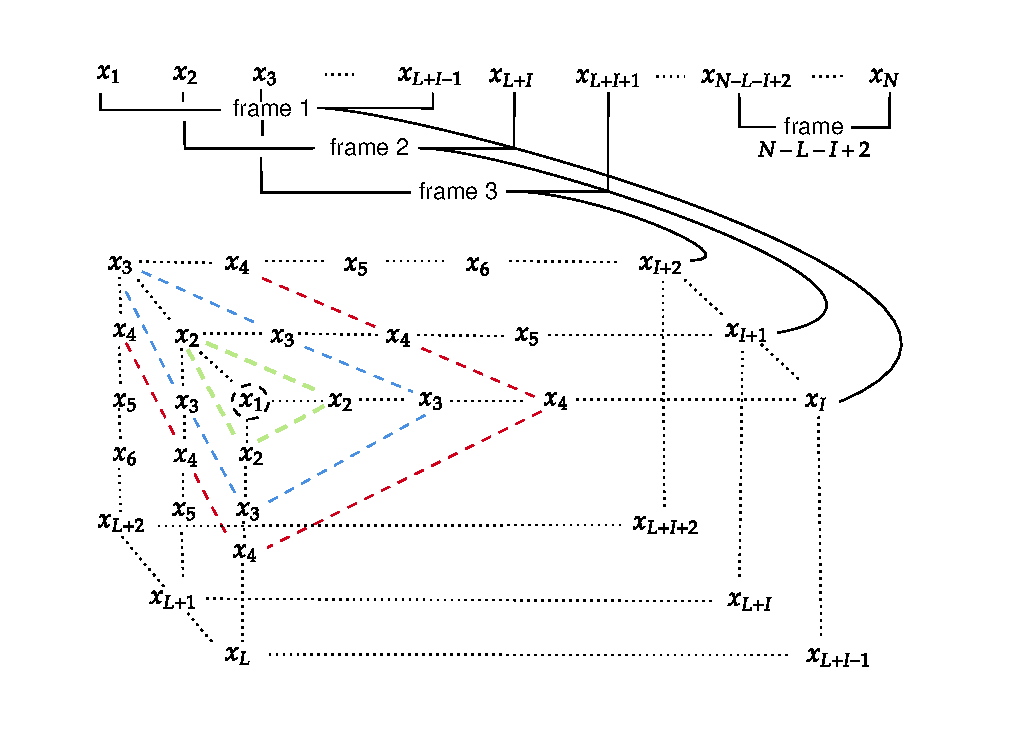
\includegraphics[width = \textwidth]{./img/tens-injection-wide}\\{}
        \vspace{-0.4cm}
        
        $I, L$ --- параметры длины окна
    \end{frame}
    
    \begin{frame}{HO-SSA: разложение и группировка}
        \begin{definition}
            $n$-ранг тензора $\calX$ $\left(\operatorname{rank}_n(\calX)\right)$ --- размерность пространства $n$-столбцов $\calX$.
        \end{definition}
        \vspace{0.2cm}
        Идея выделения сигнала: приближение $\calX$ тензором $\widetilde{\calX}$ меньших $n$-рангов.\\ \vspace{0.3cm}
        \bluetext{Способы приближения меньшими рангами:}
        \begin{enumerate}
            \item \bluetext{Усечение HOSVD:}
            \[
                \hspace{-0.5cm}
                \calX = \sum_{i=1}^{d_1}\sum_{l=1}^{d_2}
                \sum_{j=1}^{d_3} \calZ_{ilj} U^{(1)}_i \circ U^{(2)}_l \circ U^{(3)}_j \longmapsto
                \sum_{i=1}^{{\color{red} R_1}}\sum_{l=1}^{{\color{red} R_2}}
                \sum_{j=1}^{{\color{red} R_3}} \calZ_{ilj} U^{(1)}_i \circ U^{(2)}_l \circ U^{(3)}_j = \widetilde{\calX}
            \]
            \item \bluetext{Higher-Order Orthogonal Iteration (HOOI):}
            \[
                \widetilde{\calX} = \operatorname{HOSVD}\left(\arg\min_{\calY}\left\|\calX - \calY \right\|_{\rmF} \right),
                \quad \operatorname{rank}_n\left(\calY\right) = R_n 
            \]
        \end{enumerate}
        \smallskip
        
        В HO-SSA $R_1=R_2=R_3=R$
    \end{frame}
    
    \begin{frame}{HO-SSA: разделимость и ранги рядов в терминах SSA}
        \begin{itemize}
            \item \bluetext{Выделение сигнала:} нахождение ранга ряда\\ \vspace{0.1cm}
            Пусть $\tS$ --- сигнал, $\bfS_L$ --- его траекторная матрица с длиной окна $L$.
            \begin{definition}[Ранг сигнала в терминах SSA]
                $\tS$ имеет ранг $R$, если $R \leqslant N/2$ и $\forall L$: $R\leqslant \min(L, N-L+1)$\\
                $\operatorname{rank}(\bfS_L)=R$
            \end{definition}
            \item \bluetext{Разделение составляющих сигнала} пусть $\tS = \tS_1 + \tS_2$,\\
            $\bfS$, $\bfS_1$, $\bfS_2$ --- траекторные матрицы этих сигналов с длиной окна $L$
            \begin{definition}[Разделимость в терминах SSA]
                Сигналы $\tS_1$ и $\tS_2$ $L$-разделимы, если существуют такие $\gI_1, \gI_2$, что
                \[
                    \bfS = \sideset{}{_{j=1}^R}\sum\nolimits \sqrt{\lambda_j} U_j V_j^{\rmT} =
                    \overbrace{\sideset{}{_{j\in \gI_1}}\sum\nolimits \sqrt{\lambda_j} U_j V_j^{\rmT}}^{\bfS_1} +
                    \overbrace{\sideset{}{_{j\in \gI_2}}\sum\nolimits \sqrt{\lambda_j} U_j V_j^{\rmT}}^{\bfS_2}
                \]
            \end{definition}
        \end{itemize}
    \end{frame}
    
        
    \begin{frame}{HO-SSA: $n$-ранги траекторного тензора}
        \begin{theorem}[О связи рангов рядов в SSA и HO-SSA]
            Пусть сигнал $\tS$ имеет ранг $R$ в терминах \textup{SSA}.\\
            Тогда для любых значений параметров $I$ и $L$ таких, что
            \[
            R \leqslant \min(I, L, N-I-L+2),
            \] 
            $\operatorname{rank}_1(\calS)=\operatorname{rank}_2(\calS)=\operatorname{rank}_3(\calS)=R$,
            где $\calS$ --- траекторный тензор $\tS$, построенный по длинам окна $I$, $L$.
        \end{theorem}
        \vspace{0.4cm}
        \begin{remark}
            Теорема позволяет использовать известные результаты о рангах сигналов из теории \textup{SSA} для
            аппроксимации траекторного тензора на шагах разложения и группировки в методе \textup{HO-SSA}.
        \end{remark}
    \end{frame}
    
    \begin{frame}{HO-SSA: разделимость}
        Пусть $\tS = \tS_1 + \tS_2$,\\ 
        $\calS$, $\calS_1$, $\calS_2$ --- траекторные тензоры этих сигналов с длинами окна $I$ и $L$
        \begin{theorem}[О связи разделимости в SSA и HO-SSA]
            \textup{HOSVD} тензора $\mathcal{S}$ можно представить в виде суммы \textup{HOSVD}
            тензоров $\calS_1$ и $\calS_2$ тогда и только тогда, когда сигналы 
            $\tS_1$ и $\tS_2$ слабо $I$- и $L$-разделимы в терминах \textup{SSA}.
        \end{theorem}
        \vspace{0.4cm}
        \begin{remark}
            Теорема позволяет выделить класс сигналов, которые можно разделить методом \textup{HO-SSA},
            а также даёт рекомендации к выбору параметров $I$ и $L$.
%            причём этот класс более узкий, чем для метода \textup{SSA}.
        \end{remark}
    \end{frame}
    
    
    \section{HOSVD-MSSA}
    \begin{frame}{HOSVD-MSSA: алгоритм}
        Пусть $\tX = \sum_{m=1}^{M} \tS_m + \tE$ --- $Q$-канальный временной ряд\\ \vspace{0.2cm}
        
        \bluetext{Параметры:} $L$ --- длина окна, $K=N-L+1$,\\
        $R$, $\gI_1,\ldots, \gI_M$ --- как в HO-SSA,\\
        $R_3$ --- число элементов разложения по третьему направлению,\\
        $\gQ_1,\ldots, \gQ_M \subseteq \{1,2,\ldots R_3\}$, $\gQ_i \cap \gQ_j = \varnothing$ --- индексы группировки по 
        третьему направлению
        \begin{itemize}
            \item \bluetext{Вложение} $\tX \overset{L}{\longmapsto} \calX\in \bbR^{L\times K \times Q}$ --- траекторный 
            тензор
            \item \bluetext{Разложение} 
            \[
            \calX = \sum_{l=1}^{d_1}\sum_{k=1}^{d_2}
            \sum_{q=1}^{d_3} \calZ_{lkp} U^{(1)}_l \circ U^{(2)}_k \circ U^{(3)}_q
            \]
            \item \bluetext{Группировка} 
            \[
            \widetilde{\calS}_m = \sum_{l\in \gI_m} \sum_{k\in \gI_m} \sum_{q\in \gQ_m}
            \calZ_{lkp} \bfU_l^{(1)} \circ \bfU_k^{(2)} \circ \bfU_q^{(3)} 
            \]
            \item \bluetext{Восстановление} усреднение сечений третьего направления $\widetilde{\calS}_m$
            по побочным диагоналям
        \end{itemize}
        
        \vspace{0.2cm}
        
        \bluetext{Результат алгоритма:} $\widetilde{\tS}_m$ --- оценка $\tS_m$
    \end{frame}
    
    \begin{frame}{HOSVD-MSSA: траекторный тензор многоканального ряда}
        $\tX$ --- многоканальный временной ряд длины $N$\\
        $L$ --- длина окна, $K=N-L+1$ 
        
        \vspace{0.4cm}
        
        \centering
        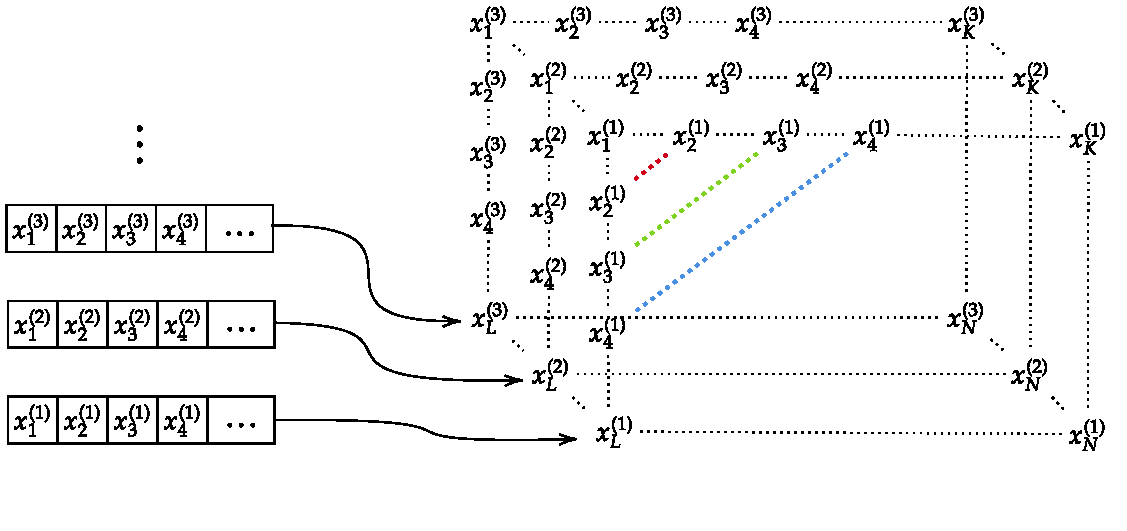
\includegraphics[width=\textwidth]{./img/mssa_injection_new}
    \end{frame}
    
    \begin{frame}{HOSVD-MSSA: $n$-ранги траекторного тензора}
        \begin{theorem}[О $n$-рангах траекторного тензора многоканального ряда]
            Пусть $\tS = \left(\tS^{(1)} : \ldots : \tS^{(Q)}\right)$, тогда справедливы следующие утверждения.
            \begin{enumerate}
                \item $\tS$ имеет ранг $R$ в терминах теории \textup{MSSA} тогда и только тогда, когда для траекторного тензора $\calS$, построенного по любой длине окна $L<N$ такой, что 
                $R \leqslant\min(L, K)$ выполняется 
                \[\operatorname{rank}_1(\calS) = \operatorname{rank}_2(\calS) = R.\]
                \item $\operatorname{rank}_3(\calS)$ равен рангу матрицы, 
                в строках которой содержатся каналы сигнала $\tS^{(q)}$.
            \end{enumerate}
        \end{theorem}
        \vspace{0.2cm}
        \begin{remark}
            Теорема позволяет использовать известные результаты о рангах сигналов из теории \textup{MSSA}
            для аппроксимации траекторного тензора по первым двум направлениям, а также даёт рекомендации к
            выбору ранга аппроксимации по третьему направлению на шагах разложения и группировки в методе \textup{HOSVD-MSSA}.
        \end{remark}
    \end{frame}
    
    \begin{frame}{HOSVD-MSSA: разделимость}
        Пусть $\tS = \tS_1 + \tS_2$, \\ 
        $\calS$, $\calS_1$, $\calS_2$ --- траекторные тензоры этих сигналов с длиной
        окна $L$\\ \vspace{0.2cm}
        $\Lambda^{(I)}(\tS) = \operatorname{span}\left\{\left(s_i^{(q)}, s_{i+1}^{(q)}, \ldots, s_{i + I - 1}^{(q)}\right)\right\}$
        \begin{theorem}[О разделимости методом HOSVD-MSSA]
            \textup{HOSVD} тензора $\calS$ можно представить в виде суммы \textup{HOSVD} тензоров $\calS_1$ и
            $\calS_2$ тогда и только тогда, когда
            $\Lambda^{(L)}(\tS_1) \perp \Lambda^{(L)}(\tS_2)$ и 
            $\Lambda^{(K)}(\tS_1)\perp\Lambda^{(K)}(\tS_2)$
        \end{theorem}
        \vspace{0.2cm}
        \begin{remark}
            Теорема позволяет выделить класс сигналов, которые можно разделить методом \textup{HOSVD-MSSA},
            а также даёт рекомендации к выбору параметра $L$.
        \end{remark}
    \end{frame}
   
    
    \section{Численные результаты}\label{sec:numerical-results}
    \begin{frame}{Численные результаты: сравнение HO-SSA с SSA}
        Пусть временной ряд имеет вид 
        \begin{gather*}
            \tX = 
            \left(s_1 + \varepsilon_1, s_2 + \varepsilon_2, \ldots, s_N + \varepsilon_N\right),
        \end{gather*}
        где $N=71$, $s_n = 30\cos(2\pi n/12)$, $\varepsilon_n$ --- шум.
        \begin{table}
            \centering
            \caption{RMSE оценки сигнала: SSA.}
            \begin{tabular}{l|cccc}
                \hline
                Вид шума &   $L=12$ &   $L=24$ &            $L=30$ &   $L=36$ \\ \hline
                Белый, $\sigma^2=25$ & 1.82 & 1.42 & \textbf{\bluetext{1.40}} & 1.42 \\ \hline
                Красный, $\delta^2 = 5$, $\varphi=0.5$ & 1.31 & 1.03 & \textbf{\bluetext{1.01}} & 1.03 \\ \hline
                Красный, $\delta^2=5$, $\varphi=0.9$ & 1.88 & 1.37 & \textbf{\bluetext{1.34}} & 1.36 \\ \hline
            \end{tabular}
        \end{table}
        
        \begin{table}
            \centering
            \caption{RMSE оценки сигнала: HO-SSA.}
            \vspace{-0.2cm}
            \begin{tabular}{l|ccccc}
                \hline
                \backslashbox{Вид шума}{\vspace*{-0.2cm}\hspace*{0.8cm}$I\times{}L$} & 19$\times$30 & 12$\times$31 &  7$\times$36  & 12$\times$37 & 12$\times$49 \\ \hline
                Белый, $\sigma^2=25$                                                 &     1.62     &     1.56     & \textbf{\bluetext{1.49}} &     1.53     &     1.63     \\ \hline
                Красный, $\delta^2 = 5$, $\varphi=0.5$                               &     1.19     &     1.14     & \textbf{\bluetext{1.08}} &     1.12     &     1.17     \\ \hline
                Красный, $\delta^2 = 5$, $\varphi=0.9$                               &     1.51     &     1.44     & \textbf{\bluetext{1.39}} &     1.42     &     1.56     \\ \hline
            \end{tabular}\label{tab:tens-hooi-ssa-cos}
        \end{table}
    \end{frame}
    
    \begin{frame}{Численные результаты: сравнение HOSVD-MSSA с MSSA и 2D-SSA}
        $\displaystyle\tX = \left(\tX_1: \ldots: \tX_Q\right),\quad \tX_q = \left(x_1^{(q)}, \ldots,
        x_N^{(q)}\right)^{\rmT}, \quad x_n^{(q)} = \hat{s}_n^{(q)} + \tilde{s}_n^{(q)} + \varepsilon_n^{(q)}$,\\
        где $\varepsilon_n^{(q)}\sim \rmN(0, 0.01)$ и независимы, модель: $s_n^{(q)} = C_q \cos(2 \pi n \omega_q + \varphi_q)$
        \begin{table}
            \centering
            \begin{tabular}{l|ccc}
                \hline
                Вид сигнала    & MSSA & HOSVD-MSSA    & 2D-SSA \\
                \hline
                Равные сигналы & \begin{tabular}{c} 0.026 \\ \hline 0.025 \end{tabular} &
                \begin{tabular}{c} 0.019 \\ \hline 0.016 \end{tabular}    &
                \begin{tabular}{c} \textbf{\bluetext{0.014}} \\ \hline \textbf{\bluetext{0.014}} \end{tabular}   \\
                \hline
                Различие амплитуд & \begin{tabular}{c} 0.029 \\ \hline 0.029 \end{tabular} &
                \begin{tabular}{c} \textbf{\bluetext{0.019}} \\ \hline \textbf{\bluetext{0.019}} \end{tabular}    &
                \begin{tabular}{c} 0.086 \\ \hline 0.083 \end{tabular}   \\
                \hline
                Линейные фазы & \begin{tabular}{c} \textbf{\bluetext{0.026}} \\ \hline \textbf{\bluetext{0.025}} \end{tabular} &
                \begin{tabular}{c} \textbf{\bluetext{0.025}} \\ \hline \textbf{\bluetext{0.025}} \end{tabular}    &
                \begin{tabular}{c} 0.117 \\ \hline 0.114 \end{tabular}   \\
                \hline
                Произвольные фазы & \begin{tabular}{c} \textbf{\bluetext{0.026}} \\ \hline \textbf{\bluetext{0.025}} \end{tabular} &
                \begin{tabular}{c} \textbf{\bluetext{0.025}} \\ \hline \textbf{\bluetext{0.025}} \end{tabular}    &
                \begin{tabular}{c} 0.034 \\ \hline 0.033 \end{tabular}   \\
                \hline
                Разделимость с $\operatorname{const}$ & \begin{tabular}{c} \textbf{\bluetext{0.017}} \\ \hline 0.025 \end{tabular}
                &
                \begin{tabular}{c} \textbf{\bluetext{0.017}} \\ \hline \textbf{\bluetext{0.019}} \end{tabular}    &
                \begin{tabular}{c} 0.023 \\ \hline 0.033 \end{tabular}   \\
                \hline
                Различие частот & \begin{tabular}{c} 0.024 \\ \hline 0.024 \\ \hline 0.024 \end{tabular} &
                \begin{tabular}{c} 0.018 \\ \hline \textbf{\bluetext{0.018}} \\ \hline \textbf{\bluetext{0.014}} \end{tabular}    &
                \begin{tabular}{c} \textbf{\bluetext{0.012}} \\ \hline 0.031 \\ \hline 0.026 \end{tabular}   \\
                \hline
                \hspace{-0.32cm}
                \begin{tabular}{l}Ортогональность\\ по каналам \end{tabular} & 
                \begin{tabular}{c} 0.031 \\ \hline 0.030 \end{tabular} &
                \begin{tabular}{c} \textbf{\bluetext{0.023}} \\ \hline \textbf{\bluetext{0.022}} \end{tabular}    &
                \begin{tabular}{c} 0.025 \\ \hline 0.024 \end{tabular}   \\
                \hline
            \end{tabular}
        \end{table}
    \end{frame}
    
    \begin{frame}{Численные результаты: смещение и дисперсия}
        $\tX = \widehat{\tS} + \widetilde{\tS} + \tE$,
        где $\hat{s}_n^{(1)} = 3$, $\hat{s}_n^{(2)} = -1.5$,
        $\tilde{s}_n^{(1)} = \cos(2\pi n / 20)$ и $\tilde{s}_n^{(2)} = 2\cos(2\pi n / 20)$, 
        а $\varepsilon_n^{(p)}\sim \rmN(0, 1)$ и независимы. 
        \begin{figure}
            \begin{minipage}[c]{0.8\textwidth}
                \hspace{-0.4cm}
                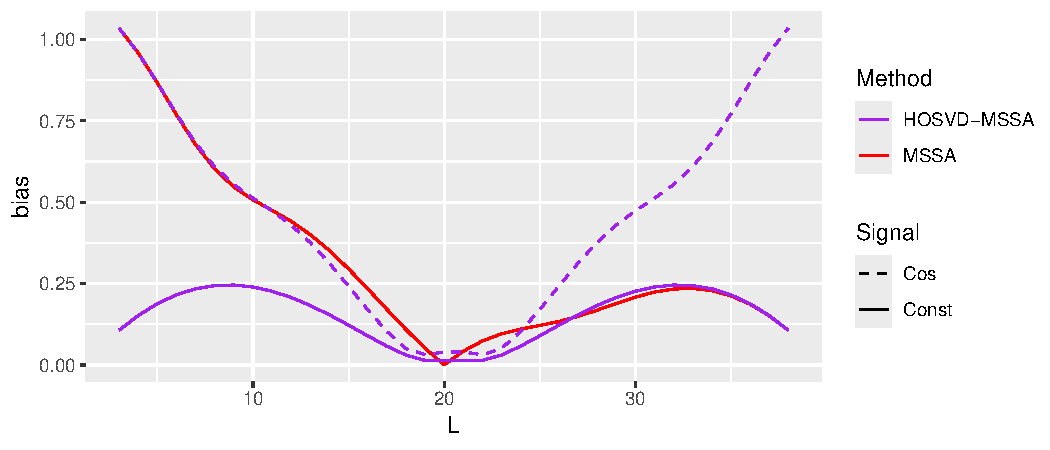
\includegraphics[width=\linewidth]{./img/approx_sep_no_noise_slides}
            \end{minipage}\hfill
            \begin{minipage}[c]{0.2\textwidth}
                \caption{Смещение оценок каждым методом (RMSE без шума)}
            \end{minipage}
            \begin{minipage}[c]{0.8\textwidth}
                \vspace{-0.1cm}
                \hspace{-0.4cm}
                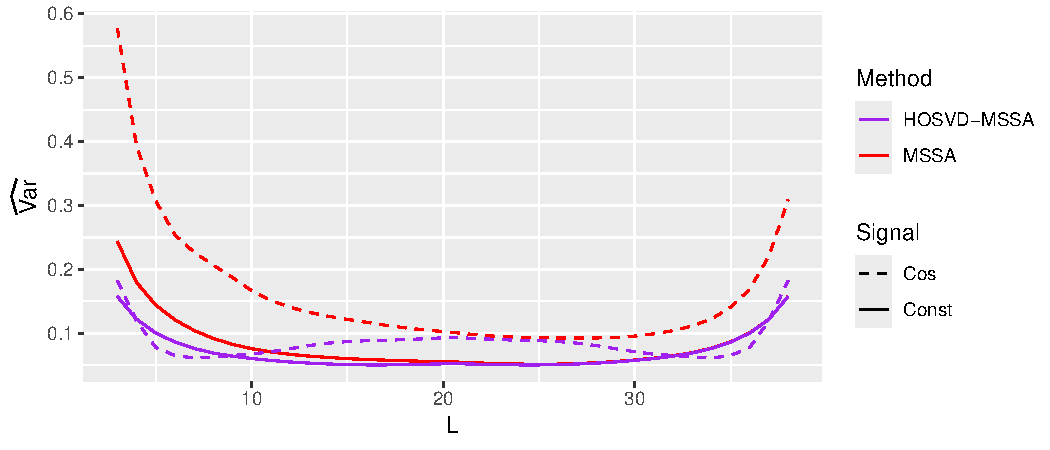
\includegraphics[width=\linewidth]{./img/approx_sep_large_noise_var}
            \end{minipage}\hfill
            \begin{minipage}[c]{0.2\textwidth}
                \caption{Дисперсии оценок каждым методом}
            \end{minipage}
        \end{figure}
    \end{frame}
    \begin{frame}{Численные результаты: сумма смещения и дисперсии}
        \begin{figure}
            \centering
            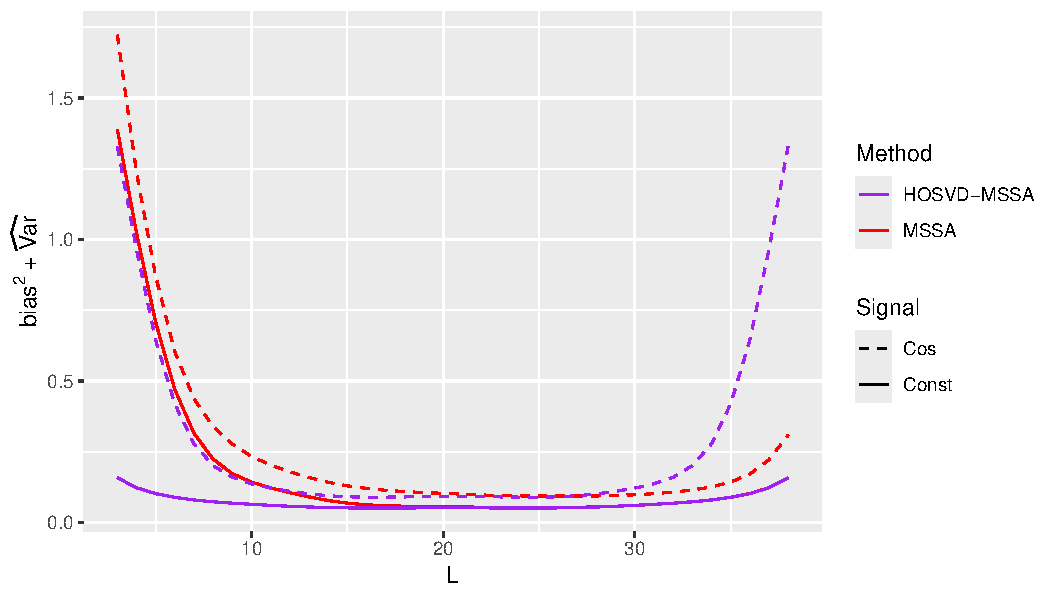
\includegraphics[width=\textwidth]{./img/approx_sep_large_noise_mse}
        \end{figure}
        Оценки методом HOSVD-MSSA могут иметь меньшую дисперсию, чем методом MSSA, однако могут проигрывать в точности за счёт
        б\'{о}льшего смещения при некоторых $L$.
    \end{frame}
   
    
    \section{Результаты}\label{sec:results}
    \begin{frame}{Результаты}
        \begin{enumerate}
            \item Свойства HO-SSA
            \begin{itemize}
                \item Критерий разделимости HO-SSA, связь с разделимостью SSA
                \item Связь рангов траекторного тензора с SSA-рангом ряда
                \item Трудоёмкость алгоритма
            \end{itemize}
            \item Свойства HOSVD-MSSA
            \begin{itemize}
                \item Критерий разделимости HOSVD-MSSA
                \item Теорема о рангах траекторного тензора, связь с MSSA-рангом и 3-ранг
                \item Утверждение о симметричности траекторного тензора относительно замены длины окна L на K
            \end{itemize}
            \item Численные выводы
            \begin{itemize}
                \item Отсутствие преимущества HO-SSA над SSA
                \item Преимущество HOSVD-MSSA над MSSA в условиях разделимости
                \item Возможное преимущество HOSVD-MSSA над MSSA в условиях приближённой разделимости для HOSVD-MSSA 
                в зависимости от соотношения смещения и дисперсии
            \end{itemize}
            \item Реализация методов HO-SSA и HOSVD-MSSA на языке R в стиле пакета Rssa (исходный код опубликован в 
            репозитории Zenodo)
        \end{enumerate}
    \end{frame}
    
    \begin{frame}[noframenumbering]{Список источников}
        \begin{thebibliography}{4}
            \bibitem{ssa1986}
            Broomhead~D.\;S., King~G.\;P.
            Extracting qualitative dynamics from experimental data //
            Physica D: Nonlinear Phenomena.~--- 1986.~--- Vol.~20, no.~2--3.~--- P.~217--236.
            
            
            \bibitem{ssa2001}
            Golyandina~N., Nekrutkin~V., Zhigljavsky~A.
            Analysis of time series structure: SSA and related techiques.
            --- Chapman \& Hall/CRC, 2001.
            
            \bibitem{mssa1986} 
            Broomhead~D.\;S., King~G.\;P.
            On the Qualitative Analysis of Experimental Dynamical Systems // 
            Nonlinear Phenomena and Chaos.~--- 1986.~--- P.~113--144.           
        \end{thebibliography}
    \end{frame}
    \begin{frame}[noframenumbering]{Трудоёмкости алгоритмов}
        \begin{itemize}
            \item \bluetext{HOSVD-SSA:} вычисление HOSVD тензора размерности $I\times L \times J$ имеет трудоёмкость порядка
            \[
                O(ILJ(\min(I, LJ) + \min(L, IJ) + \min(J, IL))).
            \]
            Если требуется вычислить только усечение HOSVD с $n$-рангами $(r_1, r_2, r_3)$, то трудоёмкость можно
            уменьшить до порядка
            \[
            O(ILJ(r_1 + r_2 + r_3)).
            \]
            \item \bluetext{HOOI-SSA:} HOOI --- итеративный алгоритм. Начальное приближение: усечение HOSVD. Трудоёмкость каждой итерации имеет порядок
            \[
                O(r_1 r_2 r_3 (I + L + J)),
            \]
            а скорость сходимости алгоритма линейная. Итого для достижения точности $\varepsilon$:
            \[
                O\left(ILJ(r_1 + r_2 + r_3) + \frac{1}{\varepsilon}r_1 r_2 r_3 (I + L + J)\right)
            \]
        \end{itemize} 
    \end{frame}
    \begin{frame}[noframenumbering]{Варианты сигналов в сравнении HOSVD-MSSA с MSSA и 2D-SSA}
        \begin{enumerate}
            \item \textbf{Равные сигналы:} $N = 44$, $P = 12$,
            \[
                \hat{s}_n^{(p)} = 2 \cos(2 \pi n / 5), \quad \tilde{s}_n^{(p)} = \cos(2\pi n /3).
            \]
            \item \textbf{Различие амплитуд:} $N = 44$, $P = 12$,
            \[
                \hat{s}_n^{(p)} = 2 c_1^{(p)} \cos(2 \pi n / 5), \quad \tilde{s}_n^{(p)} = c_2^{(p)}\cos(2\pi n /3).
            \]
            \item \textbf{Линейные фазы:} $N = 44$, $P = 12$,
            \[
                \hat{s}_n^{(p)} = 2 c_1^{(p)} \cos(2 \pi n / 5 + p \pi / 6),
                \quad \tilde{s}_n^{(p)} = c_2^{(p)}\cos(2\pi n /3 + p \pi / 9).
            \]
            \item \textbf{Произвольные фазы:} $N = 44$, $P = 12$,
            \[
                \hat{s}_n^{(p)} = 2 c_1^{(p)} \cos(2 \pi n / 5 + \varphi_1^{(p)}),
                \quad \tilde{s}_n^{(p)} = c_2^{(p)}\cos(2\pi n /3 + \varphi_2^{(p)}).
            \]
            \item \textbf{Разделимость с константой:} $N = 44$, $P = 12$,
            \[
                \hat{s}_n^{(p)} = 3 c_1^{(p)},
                \quad \tilde{s}_n^{(p)} = c_2^{(p)}\cos(2\pi n /3).
            \]
            \item \textbf{Различие частот:} $N = 59$, $P = 12$,
            \[
                \hat{s}_n^{(p)} = 2 \cos(2 \pi n / 5), \quad
                \tilde{s}_n^{(p)} = \begin{cases}
                    \cos(2\pi n /3), & 1 \leqslant p \leqslant 10,\\
                    0.4 \cos(2 \pi n / 6), & 11 \leqslant p \leqslant 12.
                \end{cases}
            \]
            \item \textbf{Ортогональность по каналам:} $N = 29$, $P = 12$,
            \[
                \hat{s}_n^{(p)} = 2 \cos(2 \pi n / 5) \cos(2 \pi p / 3), \quad
                \tilde{s}_n^{(p)} = 0.5 \cos(2\pi n /3) \cos(2 \pi p / 6).
            \]
        \end{enumerate}
    \end{frame}
\end{document}
